\subsection{User table}\label{subsec:user-table}

\texttt{
    CREATE TABLE public."user" \\
    ( \\
    id integer NOT NULL, \\
    name character varying(50) NOT NULL, \\
    email character varying(50) NOT NULL, \\
    created\_date character varying(50), \\
    updated\_date character varying(50), \\
    PRIMARY KEY (id), \\
    CONSTRAINT name\_unique UNIQUE (name), \\
    CONSTRAINT email\_unique UNIQUE (email) \\
    ); \\
    \\
    ALTER TABLE IF EXISTS public."user" \\
    OWNER to postgres; \\
}

\subsection{Event table}\label{subsec:event-table}

\texttt{
    CREATE TABLE public.event \\
    ( \\
    id integer NOT NULL,\\
    title character varying(50) NOT NULL,\\
    date character varying(50) NOT NULL,\\
    created\_date character varying(50),\\
    updated\_date character varying(50),\\
    PRIMARY KEY (id),\\
    CONSTRAINT title\_date UNIQUE (title, date)\\
    );\\
    \\
    ALTER TABLE IF EXISTS public.event\\
    OWNER to postgres;\\
}

\subsection{Ticket table}\label{subsec:ticket-table}

\texttt{
    CREATE TABLE public.ticket \\
    ( \\
    id integer NOT NULL,\\
    user\_id integer NOT NULL,\\
    event\_id integer NOT NULL,\\
    place integer NOT NULL,\\
    category character varying(30) NOT NULL,\\
    created\_date character varying(50),\\
    updated\_date character varying,\\
    PRIMARY KEY (id),\\
    CONSTRAINT unique\_event\_id\_place UNIQUE (event\_id, place),\\
    CONSTRAINT foreign\_key\_user\_id FOREIGN KEY (user\_id)\\
    REFERENCES public."user" (id) MATCH SIMPLE\\
    ON UPDATE NO ACTION\\
    ON DELETE NO ACTION\\
    NOT VALID,\\
    CONSTRAINT foreign\_key\_event\_id FOREIGN KEY (event\_id)\\
    REFERENCES public.event (id) MATCH SIMPLE\\
    ON UPDATE NO ACTION\\
    ON DELETE NO ACTION\\
    NOT VALID\\
    );\\
    \\
    ALTER TABLE IF EXISTS public.ticket\\
    OWNER to postgres;\\
}

\subsection{Database entity relations}\label{subsec:database-entity-relations}

\begin{figure}[h]
    \centering
    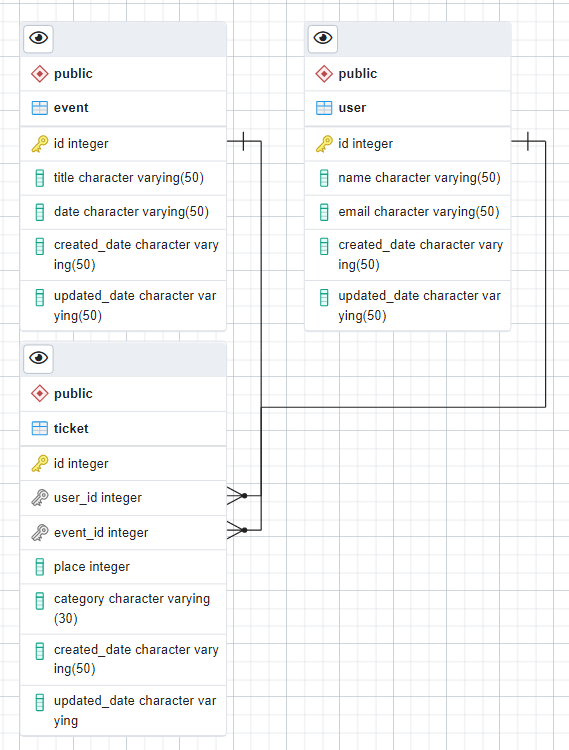
\includegraphics[width=0.8\textwidth]{images/database_relations}
    \caption{Entities relation in the database}
    \label{fig:db_relations}
\end{figure}

\subsection{Trigger for update time on UPDATE}\label{subsec:trigger}

Trigger function looks like:

\texttt{
    CREATE OR REPLACE FUNCTION public.set_update_time() \\
    RETURNS trigger \\
    LANGUAGE 'plpgsql' \\
    VOLATILE \\
    COST 100 \\
    AS $BODY$ \\
    BEGIN \\
    new.updated\_time = CURRENT\_TIME(2); \\
    RETURN new; \\
    END; \\
    $BODY$; \\
}

Trigger looks like:

\texttt{
    CREATE TRIGGER set\_update\_time\_on\_update \\
    BEFORE UPDATE OF id, name, email, created\_date, updated\_date \\
    ON public."user" \\
    FOR EACH ROW \\
    EXECUTE FUNCTION public.set\_update\_time(); \\
}

